\clearpage
\section{Results \& Discussion}
\label{sec:Results}


Succeeding the implementation phase the results of the simulation framework had to be analyzed. Due
to the complexity and high dimensionality of the problem, a focus was made on specific aspects of
the simulation.

\subsection{Simulation Result}
\label{sub_sec:Results/Results}

\begin{figure}[htbp]
  \centering
  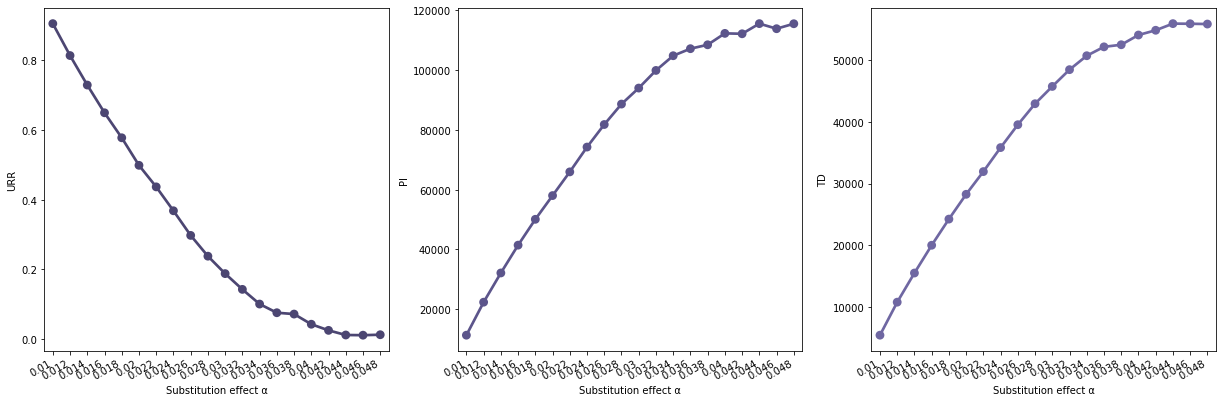
\includegraphics[width=\linewidth]{./Figures/alpha.png}
  \caption{Effects of alpha for performance metrics}
  \label{fig:Alpha}
\end{figure}

Starting with the effect of the Substitution effect $\alpha$. The Figure \ref{fig:Alpha} shows the
metrics defined in Section \ref{sub_sec:Method/Metrics} in order. For this evaluation the capacity
was set to $C = 5$, leading to a higher importance of the Substitution effect. A clear dependency
of the value of alpha to a higher performing car-sharing network can be seen. However, the curves
also indicate that the impact of the parameter decreases with larger values and the random
signal, that is due to the random nature of the simulation environment, increases.

\begin{figure}[htbp]
  \centering
  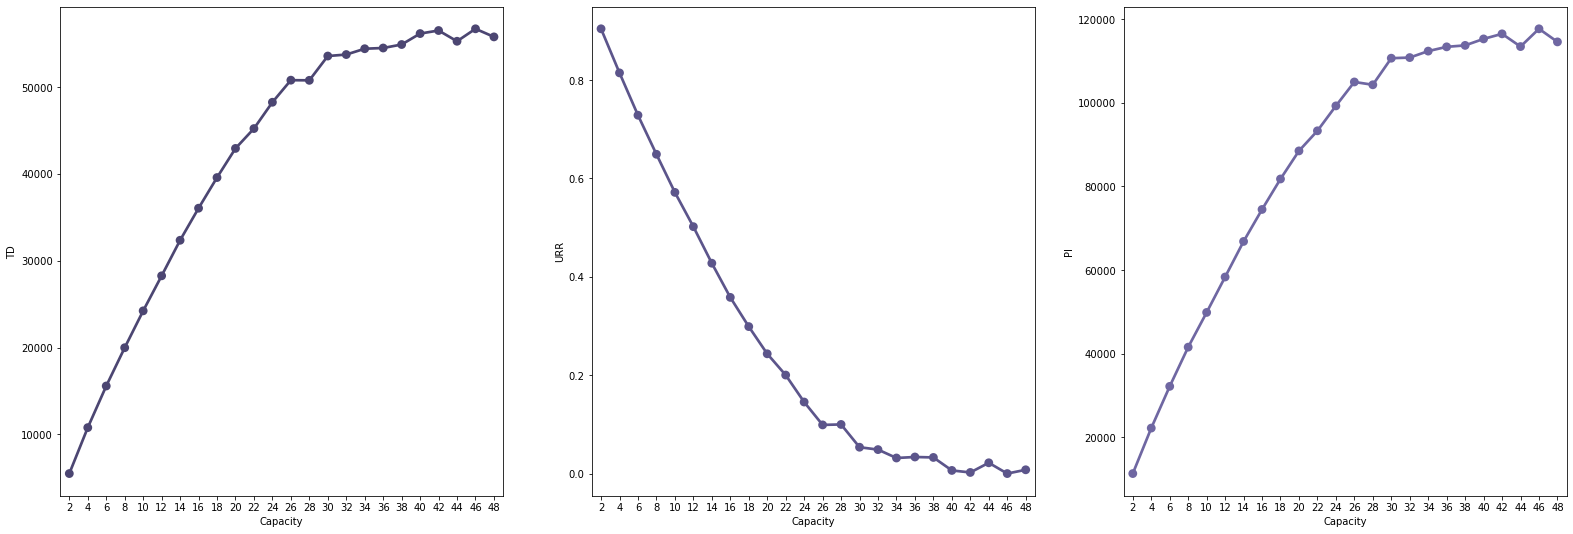
\includegraphics[width=\linewidth]{./Figures/capacity.png}
  \caption{Effects of capacity for performance metrics}
  \label{fig:Capacity}
\end{figure}

A very similar effect can be seen in Figure \ref{fig:Capacity} with the parameter $C$,
the capacity at each station. For these the alpha value has been set to $\alpha = 0.05$ 
to decrease the effect of that parameter. From an operational standpoint an optimal
fleet capacity could be determined by averaging the metrics over multiple runs
and define a threshold below which the increase in overall performance with regard to the
increase in fleet size provides no added value to the network.

\begin{figure}[htbp]
  \centering
  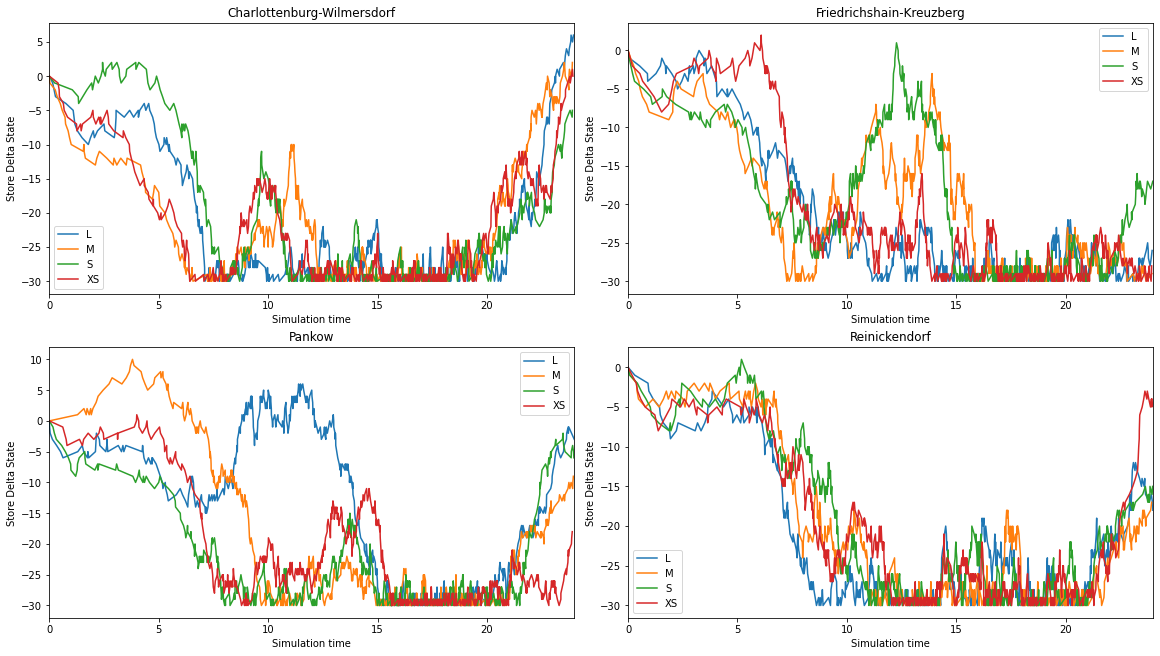
\includegraphics[width=\linewidth]{./Figures/delta-func.png}
  \caption{$\Delta_s(t, c)$ for a simulation with $\alpha=0.003, C=30$}
  \label{fig:DeltaFunc}
\end{figure}

Lastly the state function of the stations $\Delta_s(t, c)$ has been plotted against the
simulation time, to get insights of the state of the station throughout the working day.
As can be seen in Figure \ref{fig:DeltaFunc}, the impact of the demand described in Figure \ref{fig:Demand}
is clearly visible. Especially during the rush hour in the late afternoon all stations
reach capacity limits, but just about manage to keep up with an unsatisfied customer rate (URR)
of just 6.50\%. 

\subsection{Discussion \& Further Research}
\label{sub_sec:Results/Discussion}

As mentioned previously the topic of simulation in a large scale network, like a car-sharing network,
is a problem with high-dimensionality, therefore providing a lot of potential further research areas.
The focus of this thesis also included to make the simulation environment as general 
as possible, such that additional research could be conducted on the same code base.

One aspect that could be of interest, is the selection of start and end stations for
each customer request. In the real world this is typically not equally distributed but
often follows traffic flows, which are among others time and location dependent.
Another potential extension of the simulation is the extension by more stations and different
areas to potentially capture an even finer understanding of the dynamics.

While training the classifier, it became apparent that the signal of the socio-demographic
data of the rental area only correlated loosely with the decision made, and feature importance
was quite low. In further research a more sophisticated classifier could be trained that
sources a dataset which directly correlates one rental to for example the age of the
customer. Due to the modularity of the simulation that model could then easily be
exchanged with the classifier trained in this thesis and used in the simulation 
environment. 

Another aspect that would be of particular interest for the simulation stage is the parameter
$\alpha$. This parameter is not controllable by the operator but inherent for a particular
customer. One could convey a study to try to estimate the real world $\alpha$ for different
deployments of a car-sharing networks empirically.
